\documentclass{beamer}
\usepackage{verbatim}
\usepackage{xcolor}
\usepackage{multirow}
\usepackage{amssymb}
\usepackage{mathtools}  
\usepackage{tikz}
\usetikzlibrary{positioning,fit}
%\usepackage{enumitem}
\usetheme{Warsaw}
\setbeamertemplate{navigation symbols}{}
\newcommand{\blue}[1]{{\color{blue} #1}}
\newcommand{\red}[1]{{\color{red} #1}}
\newcommand{\grn}[1]{{\color{green} #1}}
\newcommand{\bluRed}[2]{{\color{blue} #1}{\color{red} #2}}
\newcommand{\qtns}[0]{\begin{center} Questions? \end{center}}
\newcommand{\nl}[1]{\vspace{#1 em}}
\newcommand{\cntrImg}[2]{\begin{center}\includegraphics[scale=#2]{#1}\end{center}}
\newcommand{\defn}[1]{{\bf #1}}
\let\emptyset\varnothing
\newcommand{\SampS}[0]{$\mathcal{S}$}

\title{Math 3070, Applied Statistics}

\begin{document}

\begin{frame}
    \begin{beamercolorbox}[rounded=true,wd=\textwidth,center]{title}
        \usebeamerfont{title}\inserttitle
    \end{beamercolorbox}
    \begin{center}
        Section 1\\
        \nl{0.5}
        August 23, 2019
    \end{center}

\end{frame}

\begin{frame}{Lecture Outline, 8/23}
    \begin{itemize}
        \item 2.1: Sample Spaces and Events
        \item Set Operations
        \item 2.2: Axioms, Interpretations, and Properties of Probability
    \end{itemize}
\end{frame}

\begin{frame}{Sample Spaces and Events, Section 2.1}
    Goal: A mathematical framework which allows one to describe experimental outcomes, extend observations into models and calculate or predict the randomness of outcomes.\\
    \nl{0.5}
    Approach:
    \begin{itemize}
        \item Section 2.1: Sample spaces and events are the foundation of most modern probabilistic models and used to describe experimental or random outcomes.
        \item Section 2.2: Probability employs a function which maps outcomes to their likelihood or chance of occuring. Note, the likelihood is often called the probability of an event.
        \item Later chapters combine probabilistic models and experimental observations to estimate models which can be used calculate or predict likelihood or probabilities, measuring randomness.
    \end{itemize}
\end{frame}

\begin{frame}{Sample Spaces and Events, Definitions}

    {\bf set}: collection of objects. Sets are denoted by curly brackets, $\{\}$. Theory of sets is \textit{topology}, used in higher level probability.\\
    \nl{0.5}
    {\bf Outcome}: values which can be observed.\\
    \nl{0.5}
    {\bf Sample Space }$\mathcal{S}, \Omega$: set all of all possible outcomes of an experiment (or random object).\\
    \nl{0.5}
    {\bf Events}: subsets of the sample space defining and denoting outcomes of experiments (or random objects). Events which have zero likeihood or probability are still events. They only need to be a subset of the sample space.  Technically, $\mathcal{S}$ is a subset of itself.\\
    \nl{0.5}
    {\bf Null Set} $\emptyset$: set with no members. Used to denoted when nothing happens or no outcome is observed. Always a subset of any set.
\end{frame}

\begin{frame}{Sample Spaces and Events, Example Coin Flip}

    Experiment: Flip a coin. Finite discrete, categorical outcomes.\\
    \nl{1}
    Sample Space $:= \{ H,T\}$\\
    \nl{0.5}
    All Events (Subsets):
    \[\emptyset, \{ H \}, \{ T\}, \{ H, T\}\]
    Note, $\{H,T\}$ is $\mathcal{S}$ and refers to a set with two members or observing any outcome in that subset. In this case, it means observing heads or tails.\\
    \nl{0.5}
    Note that outcomes and events in this framework have different meanings. The next example will meant to explain why.
\end{frame}


\begin{frame}{Sample Spaces and Events, Example Two Coin Flips}

    Experiment: Flip 2 coins. Finite discrete, categorical outcomes.\\
    \nl{1}
    Sample Space $:= \mathcal{S} = \{ (H,H),(T,H),(H,T), (T,T)\}$\\
    \nl{0.5}
    Note, denoting the outcome of each coin as (coin 1, coin 2).\\
    \nl{0.5}
    The space of all events is has an annoying number of members, $2^4 = 16$. Generally, sample spaces with $n$ outcomes have $2^n$ events.\\
    \nl{0.5}
    All Events (Subsets):
    \[\emptyset, \{ (H,H) \}, \{ (H, T)\}, \{ (T, H)\}, \{ (T, H)\},\]
    \[\{(H,H),(H,T)\}, \ldots, \{ (H,H),(T,H),(H,T), (T,T)\}\]
\end{frame}

\begin{frame}{Sample Spaces and Events, Example Two Coin Flips}

    Listing out all events is nothing more than a long excerise.  A major benefit provided by distingushing events and outcomes is the ability to describe outcomes written in english in mathematical notation, explained in the following examples.\\
    \begin{center}
        "first coin lands on heads" = $\{(H,T),(H,H)\}$\\
        \nl{0.5}
        "coins have different outcomes" = $\{(H,T),(T,H)\}$
    \end{center}
    English statements can be accurately translated into events and inserted into mathematical  (specifically probabilistic) statements.
    \[\text{English} \rightarrow \text{Probability} \rightarrow \text{Calculus} \rightarrow \text{Knowledge} \rightarrow \$\]
    \qtns
\end{frame}

\begin{frame}{Set Operations (on Events), Definitions}

    \begin{itemize}
        \item {\bf Simple Event}: event with only one outcome. Example: $\{H\};\{T\}$.
        \item {\bf Compound Event}: event more than one outcome. Example: $\{H,T\},\{(H,T),(T,H)\}$; "coins have different outcomes".
        \item {\bf Complement} of an event $A$, denoted by $A'$: the set of all outcomes in \SampS, but not the event $A$.
        \item {\bf Union} of two events $A$ and $B$, denoted by $A\cup B$: the set of all outcomes which are in either $A$, $B$ or both.
        \item {\bf Intersection} of two events $A$ and $B$, denoted by $A\cap B$: the set of all outcomes which are in both $A$ and $B$.
        \item {\bf Difference} of two events $A$ and $B$, denoted by $A\setminus B$ or $A-B$: the set of all outcomes which are in $A$, but not $B$. Order matters. Note, $A' = \mathcal{S}\setminus A$.
        \item Sets $A$ and $B$ are {\bf disjoint} if $A\cap B = \emptyset$.
    \end{itemize}
\end{frame}

\begin{frame}{Set Operations (on Events), Example Two Coin Flips}

    Consider the two coin flip example.
    \[\mathcal{S} = \{ (H,H),\blue{(T,H)},(H,T), \blue{(T,T)}\}\]
    \begin{center}
        $A =$ "first coin lands on heads" = $\{\red{(H,T)},(H,H)\}$\\
        \nl{0.5}
        $B=$ "coins have different outcomes" = $\{\red{(H,T)},(T,H)\}$
    \end{center}
    \hrule
    \nl{0.5}
    \[A' = \{ \blue{(T,H), (T,T)} \} = \text{ "first coin lands on tails"}\]
    \hrule
    \nl{0.5}
    \[A\cap B = \{ \red{(H,T)}\} =\]
    \[ \text{ "first coin lands on heads and the coins have different outcomes"}\]
    \hrule
    \nl{0.5}
    \[A\cup B = \{ (H,T), (H,H), (T,H)\} =\]
    \[ \text{ "first coin lands on heads or the coins have different outcomes"}\]
\end{frame}

\begin{frame}{Set Operations (on Events), Comments and Questions}

    \begin{itemize}
        \item Translating english statements into probabilistic statements is often the most difficult part of this class, but is one of the most used skills.
        \item "\blue{not} event $A$" translates into $A\blue{'}$.
        \item "event $A$ \red{or} event $B$" translates into $A\red{\cup}B$.
        \item "event $A$ \grn{and} event $B$" translates into $A\grn{\cap}B$.
        \item $(A')' = A$
        \item Sometimes it's easier to consider $A'$ instead of $A$.
    \end{itemize}
    \qtns
\end{frame}

\begin{frame}{DeMorgan's Laws}
    The following two identities are known as DeMorgan's laws:
    \begin{align*}
        (A \cap B)' & = A' \cup B' \\
        (A \cup B)' & = A' \cap B'
    \end{align*}
    They also extend to three or more events:
    \begin{align*}
        (A \cap B \cap C)' & = A' \cup B' \cup C' \\
        (A \cup B \cup C)' & = A' \cap B' \cap C'
    \end{align*}
\end{frame}

\begin{frame}{DeMorgan's Laws, Explanation}
    \begin{center}
        \begin{tabular}{cc}
            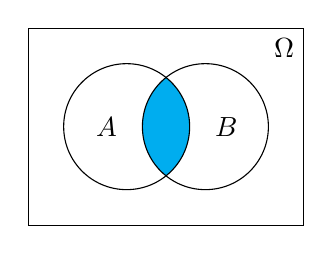
\begin{tikzpicture}[scale=.5]
                \def\firstcircle{(180:1cm) circle (1.6cm)}
                \def\secondcircle{(0:1cm) circle (1.6cm)}
                \begin{scope}
                    \clip \firstcircle;
                    \fill[cyan] \secondcircle;
                \end{scope}
                \draw \firstcircle node[text=black,left] {$A$};
                \draw \secondcircle node [text=black,right] {$B$};
                \draw (-3.5,-2.5) rectangle (3.5,2.5);
                \node at (3,2) {$\Omega$};
            \end{tikzpicture}
                       &
            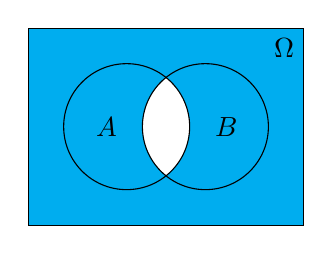
\begin{tikzpicture}[scale=.5]
                \def\firstcircle{(180:1cm) circle (1.6cm)}
                \def\secondcircle{(0:1cm) circle (1.6cm)}
                \def\mainrect{(-3.5,-2.5) rectangle (3.5,2.5)}
                \begin{scope}[even odd rule]
                    \fill[cyan] \mainrect \firstcircle;
                \end{scope}
                \begin{scope}[even odd rule]
                    \fill[cyan] \mainrect \secondcircle;
                \end{scope}
                \draw \firstcircle node[text=black,left] {$A$};
                \draw \secondcircle node [text=black,right] {$B$};
                \draw \mainrect;
                \node at (3,2) {$\Omega$};
            \end{tikzpicture} \\
            $A \cap B$ & $(A \cap B)'$
        \end{tabular}
    \end{center}

    \begin{center}
        \hspace*{-.5cm}\begin{tabular}{ccc}
            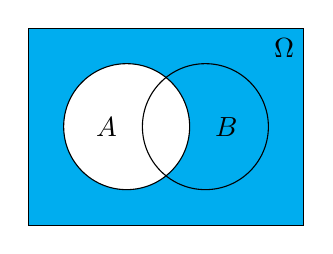
\begin{tikzpicture}[scale=.5]
                \def\firstcircle{(180:1cm) circle (1.6cm)}
                \def\secondcircle{(0:1cm) circle (1.6cm)}
                \def\mainrect{(-3.5,-2.5) rectangle (3.5,2.5)}
                \fill[cyan, even odd rule] \firstcircle \mainrect;
                \draw \firstcircle node[text=black,left] {$A$};
                \draw \secondcircle node [text=black,right] {$B$};
                \draw (-3.5,-2.5) rectangle (3.5,2.5);
                \node at (3,2) {$\Omega$};
            \end{tikzpicture}
                 &
            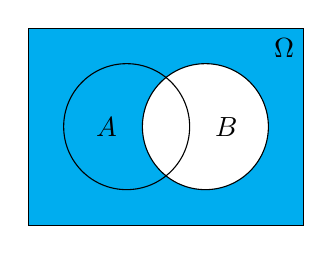
\begin{tikzpicture}[scale=.5]
                \def\firstcircle{(180:1cm) circle (1.6cm)}
                \def\secondcircle{(0:1cm) circle (1.6cm)}
                \def\mainrect{(-3.5,-2.5) rectangle (3.5,2.5)}
                \fill[cyan, even odd rule] \secondcircle \mainrect;
                \draw \firstcircle node[text=black,left] {$A$};
                \draw \secondcircle node [text=black,right] {$B$};
                \draw \mainrect;
                \node at (3,2) {$\Omega$};
            \end{tikzpicture}
                 &
            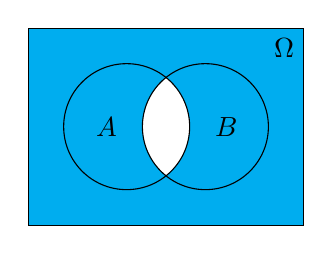
\begin{tikzpicture}[scale=.5]
                \def\firstcircle{(180:1cm) circle (1.6cm)}
                \def\secondcircle{(0:1cm) circle (1.6cm)}
                \def\mainrect{(-3.5,-2.5) rectangle (3.5,2.5)}
                \begin{scope}[even odd rule]
                    \fill[cyan] \mainrect \firstcircle;
                \end{scope}
                \begin{scope}[even odd rule]
                    \fill[cyan] \mainrect \secondcircle;
                \end{scope}
                \draw \firstcircle node[text=black,left] {$A$};
                \draw \secondcircle node [text=black,right] {$B$};
                \draw \mainrect;
                \node at (3,2) {$\Omega$};
            \end{tikzpicture} \\
            $A'$ & $B'$ & $A' \cup B'$
        \end{tabular}
    \end{center}
\end{frame}

\begin{frame}{DeMorgan's Law, questions}
    DeMorgan's Law can be useful when simplifying calculations.

    \qtns
\end{frame}

\begin{frame}{Interpretation of Probability, Section 2.2}

    In practical settings, the probability of an event is the relative frequency as the sample size become arbitrarily large, the \textit{frequentist} perspective. This is different from $\hat{p}$ which depends on the sample. Typically, the probability of a real event is hard or impossible to measure, but can be decently modeled.
\end{frame}

\begin{frame}{Axioms}

    \begin{center}
        Axioms
    \end{center}
    Given a Sample Space \SampS, $P$ is a function whose inputs are events of \SampS, and outputs are numbers between 0 and 1. These axioms aim to model the likelihood or chance of any event occuring. $\blue{P}(\red{A})$ is the \blue{probability} of \red{event A}. $P$ must follow the following axioms.
    \begin{enumerate}
        \item For any event $A$, $P(A) \geq 0$.
        \item $P(\mathcal{S})=1$.
        \item If $A_1, A_2, \ldots $ is an infinite collection of disjoint events, then
              \[P(A_1 \cup A_2 \cup \ldots) = \sum_{i=1}^\infty P(A_i).\]
    \end{enumerate}
    Caution: Axiom 3 only works with disjoint sets.
\end{frame}

\begin{frame}{Properties of Probability}

    Proposition: $P(\emptyset) = 0$.
    \begin{enumerate}
        \item $\emptyset \cap \emptyset = \emptyset$. Disjoint.
        \item $\emptyset \cup \emptyset \cup \ldots = \emptyset$.
        \item Axiom 3: $P(\emptyset \cup \emptyset \cup \ldots) = P(\emptyset) + P(\emptyset) + P(\emptyset) + \ldots$
        \item If $P(\emptyset) > 0$, then Axiom 2 is false. Observe, $\mathcal{S} = \mathcal{S} \cup \emptyset \cup \emptyset \ldots$ and $\emptyset\cap \mathcal{S} = \emptyset$, disjoint. Axiom 3 imples $P(\mathcal{S}) = P(\mathcal{S}) + P(\emptyset) + P(\emptyset) + \ldots > 1$.
        \item It must be true that $P(\emptyset)=0$ uphold axiom 2.
    \end{enumerate}
    Important use: the empty set is disjoint with all sets. This allows Axiom 3 to used with finite disjoint set by unioning infinitely many $\emptyset$ to them.

\end{frame}

\begin{frame}{Properties of Probability}

    Proposition: $P(A') = 1 - P(A)$
    \begin{enumerate}
        \item $A \cap A' = \emptyset$. Disjoint.
        \item $A \cup A' = \mathcal{S}$.
        \item Axioms 2 and 3: \[1 = P(\mathcal{S}) = P(A \cup A') = P(A) + P(A')\]
    \end{enumerate}
    Useful when simplifying calculations.\\
    \nl{0.5}
    Proposition: $P(A) \leq 1$
    \begin{enumerate}
        \item By Axiom 1, $P(A), P(A') \geq 0$.
        \item $1 = P(A) + P(A') \geq P(A)$.
    \end{enumerate}
    All probabilities of events are between 0 and 1.
\end{frame}

\begin{frame}{Probability of a Union of Two Events}
    \begin{block}{}
        $P(A\cup B)=P(A)+P(B)-P(A \cap B)$ for any events $A, B$.
    \end{block}
    Intuition: To find the probability of $A \cup B$, we add the probabilities of $A$ and $B$, but then we have double counted the intersection $A \cap B$, so we have to subtract that. In this analogy, we want to measure the 

    \vspace{.1cm}
    \begin{center}
        \begin{tabular}{c}
            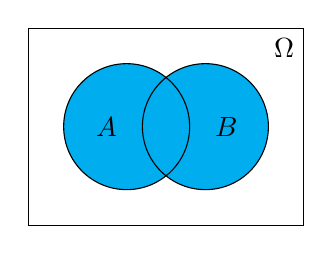
\begin{tikzpicture}[scale=.5]
                \def\firstcircle{(180:1cm) circle (1.6cm)}
                \def\secondcircle{(0:1cm) circle (1.6cm)}
                \def\mainrect{(-3.5,-2.5) rectangle (3.5,2.5)}
                \fill[cyan] \firstcircle \secondcircle;
                \draw \firstcircle node[text=black,left] {$A$};
                \draw \secondcircle node [text=black,right] {$B$};
                \draw (-3.5,-2.5) rectangle (3.5,2.5);
                \node at (3,2) {$\Omega$};
            \end{tikzpicture} \\
            $A \cup B$
        \end{tabular}
    \end{center}
\end{frame}

\begin{frame}{Probability of a Union of Two Events}
    \begin{block}{}
        $P(A\cup B)=P(A)+P(B)-P(A \cap B)$ for any events $A, B$.
    \end{block}

    Proof: We may write $A\cup B$ as a union of two disjoint events:
    $$A\cup B = A \cup (B - (A \cap B))$$
    Therefore,
    \begin{align*}
        P(A\cup B) & = P(A \cup (B - (A \cap B))) \\
                   & = P(A) + P(B - (A \cap B))   \\
                   & = P(A) + P(B) - P(A\cap B)
    \end{align*}

    \vspace{.1cm}
    \hspace*{-.3cm}\begin{tabular}{ccc}
        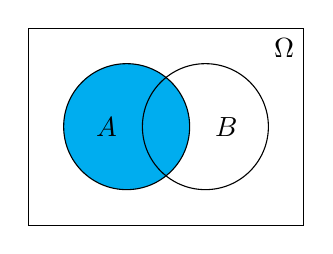
\begin{tikzpicture}[scale=.5]
            \def\firstcircle{(180:1cm) circle (1.6cm)}
            \def\secondcircle{(0:1cm) circle (1.6cm)}
            \def\mainrect{(-3.5,-2.5) rectangle (3.5,2.5)}
            \fill[cyan] \firstcircle ;
            \draw \firstcircle node[text=black,left] {$A$};
            \draw \secondcircle node [text=black,right] {$B$};
            \draw (-3.5,-2.5) rectangle (3.5,2.5);
            \node at (3,2) {$\Omega$};
        \end{tikzpicture}
                                   &
        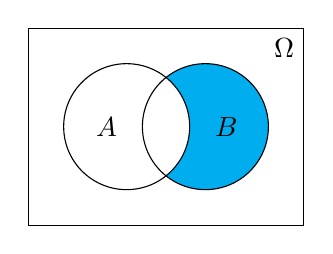
\begin{tikzpicture}[scale=.5]
            \def\firstcircle{(180:1cm) circle (1.6cm)}
            \def\secondcircle{(0:1cm) circle (1.6cm)}
            \def\mainrect{(-3.5,-2.5) rectangle (3.5,2.5)}
            \begin{scope}
                \clip \secondcircle;
                \fill[cyan, even odd rule] \firstcircle \mainrect;
            \end{scope}
            \draw \firstcircle node[text=black,left] {$A$};
            \draw \secondcircle node [text=black,right] {$B$};
            \draw (-3.5,-2.5) rectangle (3.5,2.5);
            \node at (3,2) {$\Omega$};
        \end{tikzpicture} &
        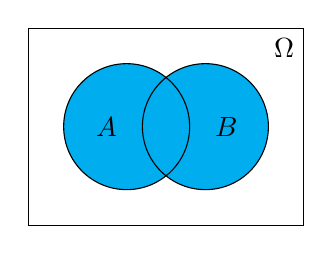
\begin{tikzpicture}[scale=.5]
            \def\firstcircle{(180:1cm) circle (1.6cm)}
            \def\secondcircle{(0:1cm) circle (1.6cm)}
            \def\mainrect{(-3.5,-2.5) rectangle (3.5,2.5)}
            \fill[cyan] \firstcircle \secondcircle;
            \draw \firstcircle node[text=black,left] {$A$};
            \draw \secondcircle node [text=black,right] {$B$};
            \draw (-3.5,-2.5) rectangle (3.5,2.5);
            \node at (3,2) {$\Omega$};
        \end{tikzpicture}                                \\
        $A$                        & $B - (A\cap B)$ & $A \cup B$
    \end{tabular}

\end{frame}

\begin{frame}{Probability of a Union of Three Events}
    \begin{block}{}
        \vspace{-.2in}\begin{align*}
            P(A \cup B \cup C) = \  & P(A)+P(B)+P(C)                         \\
                                    & -P(A \cap B)-P(A \cap C) - P(B \cap C) \\
                                    & + P(A\cap B\cap C)
        \end{align*}
    \end{block}

    Intuition: To find the probability of $A \cup B \cup C$, we add the probabilities of the events $A$, $B$, and $C$ and subtract the overlap of each pair; but then we've subtracted the three-way overlap $A \cap B \cap C$ one too many times, so we add it back.
    \begin{center}
        Nice to know, but rarely used.
    \end{center}
\end{frame}

\begin{frame}{Properties of Probability, Summary}
    \begin{block}{Axioms}
        \begin{enumerate}
            \item For any event $A$, $P(A) \geq 0$.
            \item $P(\mathcal{S})=1$.
            \item If $A_1, A_2, \ldots $ is an infinite collection of disjoint events, then
                  $P(A_1 \cup A_2 \cup \ldots) = \sum_{i=1}^\infty P(A_i)$.
        \end{enumerate}
    \end{block}
    \begin{block}{Propositions}
        \begin{enumerate}
            \item $P(\emptyset)=0$
            \item If $A_1, A_2, \ldots, A_n $ is an finite collection of disjoint events, then
            $P(A_1 \cup A_2 \cup \ldots \cup A_n) = \sum_{i=1}^n P(A_i)$.
            \item $P(A') = 1 -P(A)$
            \item For any events $A$ and $B$, \\$P(A\cup B) = P(A) + P(B) - P(A\cap B)$.
        \end{enumerate}
    \end{block}
\end{frame}

\begin{frame}{Interpretation of Probability}

    Under this model of the probability of an event is the proportion of times it should occur in a very large sample. This is different from $\hat{p}$ which depends on the sample. Typically, the probability of a real event is hard or impossible to measure, but can be decently modeled.
\end{frame}

\begin{frame}{Equally Likely Outcomes}
    Given a finite sample space $\Omega$, one of the simplest ways to define a probability measure is to assume that the outcomes are \\{\bf equally likely}:
    $$P(A) = \frac{\# A}{\# \Omega} = \frac{\text{number of outcomes in $A$}}{\text{number of outcomes in $\Omega$}}$$
    
    \begin{example}
    Suppose we roll a fair six-sided die. Let $\Omega=\{1,2,3,4,5,6\}$, and let $A=\{2,4,6\}$ be the event that we roll an even number. Then
    $$P(A)=\frac{\# A}{\#\Omega}=\frac36=\frac12=.5$$
    \end{example}
    It is not always reasonable to assume the outcomes are equally likely. %For example, in the three-component system example, we found $P(SFS)=.378$ but $P(FSF)=.012$.
    \qtns
    \end{frame}

    \begin{frame}{Disjoint Sum Example, Rolling Two Dice}
        
        Problem: What is the probability that a roll of two fair die lands on two exactly once?\\
        \nl{0.5}
        Notation: $(X_1,X_2)$, \\
        $X_1 =$ value of first die, \\$X_2 =$ value of second die.\\
        \nl{0.5}
        \begin{center}
        $\mathcal{S} = \{(1,1), (1,2), (1,3) \ldots (6,5), (6,6)\}$, 36 pairs
        \end{center}
        Since the dice are fair, each pair is equally likely, all have probability of $1/36$.
    \end{frame}

    \begin{frame}{Disjoint Sum Example, Rolling Two Dice}
        \begin{enumerate}
            \item Event $A =$ "two rolled exactly once".
            \item Event $B =$ "first die is two, second is not".
            \item $B = \{ (2,1),(2,3),(2,4),(2,5),(2,6) \}, \red{P(B) = 5/36}$
            \item Event $C =$ "second die is two, first is not".
            \item $C = \{ (1,2),(3,2),(4,2),(5,2),(6,2) \}, \blue{P(C) = 5/36}$
            \item $A = \red{B} \cup \blue{C}$
            \item $\blue{C} \cap \red{B} = \emptyset$, disjoint.
            \item Sum of disjoint sets, $P(A) = \red{P(B)} + \blue{P(C)} = 10/36 = 5/18$
        \end{enumerate}

    \end{frame}

    \begin{frame}{Complement Example, Rolling Two Dice}
        
        Problem: What is the probability that two fair dice do not land on the same number?\\
        
        \begin{enumerate}
            \item Event $A =$ "dice land on different numbers".
            \item Event $A' =$ "dice land the same number".
            \item $A' = \{ (1,1), (2,2), \ldots, (6,6) \}$.
            \item $P(A') = 6/36 = 1/6$.
            \item $P(A) = 1 - P(A') = 1 - 1/6 = 5/6$.
        \end{enumerate}
    \end{frame}

    \begin{frame}{Nondisjoint Example, Rolling Two Dice}
        
        Problem: What is the probability that two fair dice show either two exactly once or two even numbers?\\
        \begin{enumerate}
            \item event $A =$ "two rolled exactly once"
            \item \red{$P(A) = 10/36$} from before.
            \item event $B = $ "rolled two even numbers"
            \item $B = \{ (2,2), (2,4), (2,6), (4,2), (4,4), (4,6), (6,2),(6,4), (6,6) \}$
            \item \blue{$P(B) = 9/36$}, 9 pairs
            \item $B\cap A = \{ (2,4), (2,6), (4,2), (6,2) \}$
            \item \grn{$P(A \cap B) = 4/36$}
            \item $P(A \cup B) = P(A) + P(B) - P(A \cap B) =$  $\red{10/36} + \blue{9/36} - \grn{4/36} =  15/36$
        \end{enumerate}
    \end{frame}

    \begin{frame}{DeMorgan's Law Example, Flipping Six Coins}
        
        Problem: Suppose a fair coin is flipped six times. What is probability that  at least one head and one tail is observed?\\
        \begin{enumerate}
            \item event $A =$ "at least one head \blue{and} tail is observed"
            \item $A= \text{"at least one head"} \blue{\cap} \text{"at least one tail"}$ 
            \item DeMorgan's Law $A' =\grn{(\text{"at least one head"})'} \blue{\cup} \red{(\text{"at least one tail"})'}$
            \item event $\red{B} = (\text{"at least one tail"})' = \text{"six heads observed"} = \{ (H,H,H,H,H,H) \}$
            \item event $\grn{C} = (\text{"at least one head"})' = \text{"six tails observed"} = \{ (T,T,T,T,T,T) \}$
            \item There are $2^6=64$ outcomes, equally likely. Events $B$ and $C$ are one outcome each so $P(B)=P(C) = 1/64$.
            \item $B$ and $C$ are disjoint, $P(B\cup C) = P(B) + P(C) = 1/32$.
            \item $P(A) = 1 - P(A') = 1 - P(\red{B} \blue{\cup} \grn{C}) =31/32$.
        \end{enumerate}
    \end{frame}

    \begin{frame}{Probability Table Example}
        
        At an intersection, cars either turn right, turn left or go straight with the following probabilities.
        \begin{center}
        \begin{tabular}{| l | r | r | r|}
            \hline
            action & left & right & straight \\
            \hline
            probability & 0.14 & 0.16 & 0.7 \\
            \hline
        \end{tabular}
    \end{center}
    What is the probability that a car turns? What is the probability that a car does not turn right?
    \begin{itemize}
        \item events $\{\text{"turn right"}\}$ and $\{\text{"turn left"}\}$ are disjoint.
        \item $P(\text{"car turns"}) = P(\text{"turn right"} \cup \text{"turn left"}) = P(\text{"turn right"}) + P(\text{"turn left"}) = 0.14 + 0.16 = 0.3$
    \end{itemize}
    \[P(\text{"does not turn right"}) = 1 -P(\text{"turn right"}) = 1 - 0.16 = 0.84\]

    \end{frame}

    \begin{frame}{Example, Census Proportions}
        Census data informs you that \blue{67\%} of households have more than one car, \grn{63\%} of households have more than one car and more than one person and \red{31\%} of households have one person. What is the probability that a randomly selected household has one person or more than one car?\\
        \nl{0.5}
        event $\blue{A} =$ "household has more than one car"\\
        \nl{0.5}
        event $\red{B} =$ "household has more than one person"\\
        \nl{0.5}
        $B' =$ "household has one person"\\
        \[P(B) = 1 - P(B') = 1 - \red{0.31} = 0.69\]
        \begin{alignat*}{3}
            P(A \cup B)  & = P(A) &+ P(B) &- \grn{P(A\cap B)}\\
                &= 0.67 &+ 0.69 &- 0.63\\
                & = 0.73
        \end{alignat*}
    \end{frame}
\end{document}